\section{Technical overview}\label{sec:overview}

This section walks through the whole argument at the level of ideas, so that the formal development in
\cref{sec:support,sec:dt,sec:main} and the proofs in the appendices can be read against a map. Nothing
here is used later; the reader who prefers to start from definitions may skip to \cref{sec:prelim}.

\subsection{The cluster-count integral and where the cost hides}\label{sec:ov-integral}

Every sublinear MST-weight algorithm in this lineage rests on one identity. For a finite $S\subset\R^2$
and a threshold $t$, let $c_S(t)$ be the number of connected components of the graph that joins two points
of $S$ when they are within distance $t$; these components are the single-linkage clusters at scale $t$.
As $t$ grows the clusters merge, each merge corresponding to one MST edge, and the Chazelle--Rubinfeld--
Trevisan identity~\cite{CRT05} writes the MST weight as the area under the resulting staircase,
\begin{equation}\label{eq:ov-integral}
  \wt(\MST(S))=\int_0^\infty\bigl(c_S(t)-1\bigr)\,dt .
\end{equation}
Estimating $\wt(\MST(S))$ thus reduces to estimating the curve $c_S(\cdot)$ at a geometric ladder of
thresholds and summing. Under the range-counting oracle we cannot see points, only counts in boxes, so the
whole problem becomes: \emph{estimate the number of single-linkage clusters at a given scale, using few
range counts.}

Counting components in sublinear time is classically done by sampling: pick a few vertices, explore their
components, and extrapolate~\cite{CRT05,CzumajSohler09}. In the geometric setting this is exactly what
costs $\Omega(\sqrt n)$. The reason is a mismatch between mass and weight. Consider a dense
$\sqrt K\times\sqrt K$ block of points together with a handful of far-flung satellites. The satellites are
a vanishing fraction of the points, so a sample of $\poly\log$ many points misses them with high
probability; yet each satellite is its own cluster across a wide range of scales and so contributes a
constant fraction of the MST weight. To see the satellites by sampling \emph{points} one must draw
$\Omega(\sqrt K)$ of them, and paying this at every scale is the $\sqrt n$ barrier of~\cite{DMOSW25}.

\subsection{The empty-cell spatial leader estimator}\label{sec:ov-leader}

Our one new primitive removes that barrier by sampling \emph{space} instead of mass. Fix a scale and lay
down a fine grid. Form the \emph{scale graph} whose vertices are the nonempty cells and whose edges join
cells that are close, so that its component count brackets $c_S$ at nearby thresholds
(\cref{sec:support-filtration}). To estimate the number of components $c$ of a graph $\Gamma$ on a known
universe $\mathcal U$ of $M$ candidate cells, run the following one-bit experiment, illustrated in
\cref{fig:leader}.

\begin{quote}
Draw a cell $X$ uniformly from $\mathcal U$, \emph{including empty cells}. If $X$ is empty, output $Z=0$.
Otherwise assign independent uniform ranks to the occupied cells and explore the component of $X$ in
$\Gamma$, stopping as soon as a cell of smaller rank than $X$ appears. Output $Z=M$ if $X$ is the
minimum-rank cell of its component (its \emph{leader}) and $Z=0$ otherwise.
\end{quote}

\begin{figure}[t]
\centering
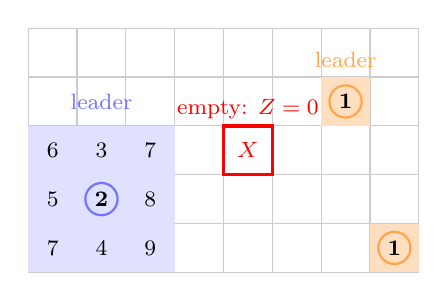
\begin{tikzpicture}[scale=0.62, every node/.style={font=\footnotesize}]
  % grid
  \draw[step=1cm, gray!40, thin] (0,0) grid (8,5);
  % a dense block (occupied cells) bottom-left
  \foreach \x/\y in {0/0,1/0,2/0,0/1,1/1,2/1,0/2,1/2,2/2} {
    \fill[blue!12] (\x,\y) rectangle (\x+1,\y+1);
  }
  % ranks in the block component (min-rank = leader)
  \node at (0.5,0.5) {7}; \node at (1.5,0.5) {4}; \node at (2.5,0.5) {9};
  \node at (0.5,1.5) {5}; \node at (1.5,1.5) {\textbf{2}}; \node at (2.5,1.5) {8};
  \node at (0.5,2.5) {6}; \node at (1.5,2.5) {3}; \node at (2.5,2.5) {7};
  \draw[blue!55,thick] (1.5,1.5) circle (0.33); % leader of the block
  % two satellites, each its own component
  \fill[orange!25] (6,3) rectangle (7,4); \node at (6.5,3.5) {\textbf{1}};
  \draw[orange!70,thick] (6.5,3.5) circle (0.33);
  \fill[orange!25] (7,0) rectangle (8,1); \node at (7.5,0.5) {\textbf{1}};
  \draw[orange!70,thick] (7.5,0.5) circle (0.33);
  % a sampled empty cell (X)
  \draw[red,very thick] (4,2) rectangle (5,3); \node[red] at (4.5,2.5) {$X$};
  \node[red] at (4.5,3.35) {empty: $Z=0$};
  \node[blue!55] at (1.5,3.5) {leader};
  \node[orange!70] at (6.5,4.35) {leader};
\end{tikzpicture}
\caption{The empty-cell leader estimator. Candidate cells are sampled uniformly from a universe that
includes empty ones (an empty sample, shown in red, returns $0$). On an occupied sample, ranks are drawn
and the unique minimum-rank cell of each component (circled) returns $Z=M$. A far satellite is one cell of
the universe like any other, so it is found with the right probability; its tiny mass never enters.}
\label{fig:leader}
\end{figure}

For any fixed ranking exactly one cell per component is its leader, so exactly $c$ of the $M$ candidates
return $M$ and the rest return $0$. Hence $\E Z=M\cdot(c/M)=c$ and $\E Z^2=M^2\cdot(c/M)=Mc$, giving the
variance bound
\begin{equation}\label{eq:ov-var}
  \E Z=c,\qquad\Var(Z)=Mc-c^2\le Mc .
\end{equation}
Two features make this the right estimator. First, its variance is governed by the \emph{component count}
$c$, not by the number of occupied cells: the satellite is one candidate among $M$ and is sampled with
probability $1/M$ regardless of how few points it holds, so the heavy tail is no longer invisible.
Second, an occupied exploration is cheap in expectation: the cell examined $j$-th in the rank order is
examined only when the start has the smallest rank among the first $j$, an event of probability $1/(j-1)$,
so an exploration touches $O(\log K)$ cells on average, the same harmonic bound that later controls the
death-time search.

\subsection{Two costs, one packing inequality, and the \texorpdfstring{$\sqrt K$}{sqrt K} bound}
\label{sec:ov-twopart}

To turn \eqref{eq:ov-var} into an algorithm we estimate $c=c_\Gamma(r)$ at each scale $r$ to an additive
accuracy $\alpha_r$ tuned so the scale-by-scale errors sum to $\eps\Wq$. A median-of-means average of the
one-bit experiment needs $O(MU/\alpha_r^2)$ trials, where $U\ge c$ is an a-priori bound on the component
count; this is the \emph{trial cost}. Separately, each occupied trial explores cells, and an exploration
can touch up to $N$ occupied cells; this is the \emph{exploration cost}. The crucial point is that these
two costs scale with different quantities, $U$ (a bound on the component count) and $N$ (the occupied-cell
count), and we account for them separately.

Both sums are collapsed by a single geometric fact about the support, the \emph{active-cover packing}
inequality $\Wq\ge b\delta/16$ (\cref{lem:packing}), where $b=\Theta(\sqrt K)$ is the number of blocks of
a canonical cover and $\delta$ their side. Intuitively, a support with $K$ cells cannot have its MST weight
concentrated too thinly: spreading $K$ cells out forces $\Wq$ up in proportion to $\sqrt K$ times the
spread. Feeding this into the geometric sum over scales turns both the trial and exploration sums into
$\Otil(\sqrt K)$, which is the content of \cref{lem:support}: the MST weight of a $K$-cell support is
$(1\pm\eta)$-estimable in $\Otil_\eta(\sqrt K+n/K)$ range counts, the additive $n/K$ being the cost of
learning $K$ itself by rejection sampling.

\subsection{From a grid support back to the point set}\label{sec:ov-reduction}

\Cref{lem:support} estimates a grid support, not the input $P$. Three steps bridge the gap, and they are
the substance of \cref{sec:dt}. Fix a guess $G\ge W$ and a clip level $L=G/K_0$ with $K_0=\ceil{n^{2/3}}$,
and split the MST weight at $L$ into a \emph{bulk} $A_L=\sum_e\min\{\abs e,L\}$ and a \emph{tail}
$B_L=\sum_e(\abs e-L)_+$.

\emph{The bulk of $P$} is estimated directly by a \emph{clipped death-time sampler}. Assign random ranks
to the vertices of a graph $H$ and let the death time $\tau(v)$ be the bottleneck (min-over-paths of the
max edge) distance from $v$ to the root or to any lower-ranked vertex; the multiset of death times equals
$\{0\}\cup\{\text{MST edge weights}\}$, so the clipped average $\abs V\cdot\E\min\{\tau,L\}$ is exactly
$A_L(H)$, with variance controlled by the clip. Running this on a locally navigable $(1+\rho)$-spanner of
$P$ gives $A_L(P)$ up to a $(1+\rho)$ factor.

\emph{The tail} is routed through a grid support. We regularize: choose a grid scale $h$ whose support has
$\Theta(K_0)$ cells (\cref{lem:kwindow}), and snap each point to its cell center. Snapping moves points by
$O(\xi L)$, which interleaves the threshold graphs of $P$ and of the support $Q$ and transfers the tail
$B_L(P)$ to $B_L(Q)$ up to an $O(\xi W)$ error. The support tail is then $B_L(Q)=\Wq-A_L(Q)$, where $\Wq$
is the support-MST weight from \cref{lem:support} and $A_L(Q)$ is another clipped death-time average, this
time on a spanner of the support.

\emph{Assembly.} Adding the bulk of $P$ to the tail of the snapped support,
\begin{equation}\label{eq:ov-assembly}
  \widehat W=\widehat A_P+\widehat\Wq-\widehat A_Q ,
\end{equation}
and choosing the internal accuracy $\xi=\Theta(\eps)$ makes every error term $O(\eps G)$. A guess $G\ge W$
is removed by a geometric search that stops at the first $G$ with $\widehat W(G)\ge G/8$, which lands in
$[W,16W)$; a final calibrated call then gives the $(1\pm\eps)$ estimate. The three estimators draw fresh
samples, so their errors are independent, and no seed is reused across thresholds.

\subsection{Realizing the spanner under a counting oracle}\label{sec:ov-wspd}

The death-time sampler needs a Euclidean $(1+\rho)$-spanner that can be navigated from a sampled vertex
using only range counts. We build it from the well-separated pair decomposition of the quadtree on
$[\Delta]^2$~\cite{CK95,HarPeled11}. Each cell gets a representative, the $z$-first point inside it, found
by binary search on counts; a spanner edge joins the representatives of each well-separated pair and
carries their exact Euclidean length, which we know because we know the representatives' coordinates. From
a vertex $u$ the incident spanner edges are enumerated by scanning the $O(\log\Delta)$ quadtree ancestors
of $u$ at which $u$ is the representative and, for each, its $O(\rho^{-2})$ well-separated partner cells.
A bottleneck Dijkstra over exact edge weights then computes $\tau(v)$ exactly, halting at the first
lower-ranked vertex after $O(\log\abs V)$ expansions in expectation. The full implementation, including a
global query budget that makes the whole call abort rarely instead of biasing any single search, is
\cref{sec:wspd}. This is the part inherited from~\cite{DMOSW25} and the one a verifier should read most
closely.

\subsection{The balance point}\label{sec:ov-balance}

The two halves meet at $K_0=\Theta(n^{2/3})$. The support estimator costs $\Otil(\sqrt K+n/K)$, minimized
over $K$ at $K=n^{2/3}$ where it is $\Otil(n^{1/3})$. The clipped death-time sampler for the bulk needs
$O(\xi^{-2}n/K_0)=O(\xi^{-2}n^{1/3})$ samples at $\Otil_\rho(1)$ counts each, again $\Otil(n^{1/3})$. The
regularization search and the support sampler are $\Otil(n^{1/3})$ as well. Every piece is $\Otil_\eps(
n^{1/3})$, and so is their sum, which is \cref{thm:main}. The matching $\Omega(n^{1/3})$ lower bound
of~\cite{DMOSW25} (\cref{sec:optimality}) shows the exponent cannot be improved.
